\section{Kapitel 1}
\subsection{Aufgabenstellung}
Um uns mit Java und der Konsole vertraut zu machen sollten wir zuerst ein Java Programm in der Konsole
schreiben, welches "Dear Prudence\dq \space ausgibt. Anschlie\ss end mit Javac Kompilieren und mit Java
ausführen. Wenn wir dies geschafft haben, sollte wir als nächstes in NetBeans ein neues Projekt erstellen
und dort das selbe Programm erneut Programmieren. 

\subsection{Anforderungsdefinition}
\begin{enumerate}
	\item Das Programm soll "Dear Prudence\dq \space auf der Konsole ausgeben.
\end{enumerate}

\subsection{Entwurf}
\begin{center}
	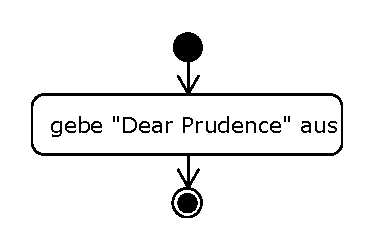
\includegraphics[width=0.4\textwidth]{uml/uml_c1_p2.pdf}
\end{center}

\subsection{Quellcode}
\subsubsection{Main.java}
\lstinputlisting[language = Java , frame = trBL , firstnumber = last , escapeinside={(*@}{@*)}]{../chapter_01/src/main/java/chapter_01/Main.java}

\subsection{Testdokumentation}
Wenn das Programm gestartet wird, sollte "Dear Prudence\dq \space auf der Konsole ausgegeben werde.
Dies war der fall.

\subsection{Benutzungshinweise}
Navigieren Sie in der Kommandozeile zum dem Ordner, wo sich die Java Datei befindet.
Danach führen sie "javac Main.java\dq \space auf. Jetzt können Sie das Programm mit "java main\dq \space
 starten. In der Konsole sollte nun "Dear Prudence\dq \space angezeigt werden.

\subsection{Anwendungsbeispiel}
Nach dem Aufruf von java Main, sollten wir folgendes sehen:
\begin{lstlisting}[frame = trBL , escapeinside={(*@}{@*)}]
[sebastian@laptop bin]$ java Main 
Dear Prudence
[sebastian@laptop bin]$ 
\end{lstlisting}